\graphicspath{{chapters/muonsim/images/}}
\chapter{Low-Energy Muon Simulation}
\label{chapter:muonsim}
The updates of the noise simulation provide one reduction of background uncertainties in the tau neutrino appearance analysis.
Another large uncertainty in the analysis is due to the limited simulation statistics of the atmospheric muon samples.

For low-energy oscillation analyses, the simulation of muons has proven difficult due to the computationally intensive simulation scheme.
Large numbers of simulated events are produced for general IceCube analysis use, although the vast majority of these background muons do not reach DeepCore.
In response, previous analyses \cite{IceCube-Oscillation2013,IceCube-Oscillation2015,IceCube-Oscillation2018,IceCubeSterile-Andrii} have developed methods to reuse data events which fail the selection as a model of the background at Final Level.
Severely limited simulated statistics from the CORSIKA generator precluded strong checks of these samples.

For the search for tau neutrinos, new background generation techniques were used to more robustly model atmospheric muons.
Two new generation schemes for low energy IceCube analyses are discussed here.
The first, briefly discussed in Section~\ref{sec:muongun_deepcore}, provided the final background sample used in the search for tau neutrinos.
The second method, discussed in Section~\ref{sec:kde_filtering}, is more experimental, but shows potential to further improve the background generation efficiency substantially for future analyses.

\section{CORSIKA Generation In DeepCore}
\label{sec:corsika_problems}
In IceCube, most simulation is produced centrally for use by the entire collaboration.
This is especially true for background simulation produced with the CORSIKA generator.

CORSIKA simulation, using the 5-component scheme discussed in Section~\ref{subsubsec:corsika}, is the most common background simulation used in IceCube.
These simulations are broken into two energy ranges based on the simulated primary particle energy in order to allow efficient generation of rare, high energy events.
These are "low energy" CORSIKA, produced with primary energies 600~GeV~$\leq E_{prim} <$~10~TeV, and "high energy" CORSIKA, with energies 10~TeV~$\leq E_{prim}~<$~100 EeV.

Unlike MuonGun, CORSIKA generation does not currently possess a method to target specific sections of the detector. 
Instead, CORSIKA muons target a cylinder of radius 800~m and length 1600~m centered on and fully enclosing the IceCube detector.
This allows uniform coverage useful for a wide range of analyses.

The centralized CORSIKA simulation in IceCube results in simulated background datasets used by all analyses in the collaboration.
The production of these sets is computationally intensive, requiring hundreds of CPU-years and GPU-years worth of processing time in order to reach sufficient statistics for all but the highest energy IceCube analyses.
The number of unweighted simulation events and required computational resources required for centralized CORSIKA sets is shown in Table~\ref{tab:corsika_stats}.
Included is the 'simulation efficiency', the average number of events produced per computational year.

\begin{equation}
\epsilon = \frac{N_{final}}{t_{CPU}+t_{GPU}}
\end{equation}

For analyses using DeepCore, the CORSIKA generation scheme results in many muons that are easily rejected during event selections.
Events which interact solely outside of the DeepCore fiducial volume are removed early by a veto algorithm discussed in Section~\ref{sec:DeepCoreFilter}, reducing the background statistics from O($10^{12}$) to O($10^6$). 
Additional cuts reduce this number further, with the GRECO selection described in Chapter~\ref{chapter:greco} removing all but 284 events from an intial sample of $8\times 10^{12}$.
These events represent nearly 10\% of the Final Level sample after weighting.

\begin{table}[]
\centering
\begin{tabular}{@{}llllll@{}}
\toprule
\multirow{2}{*}{Generator} & \multicolumn{2}{c}{Sim. Req.} & \multicolumn{2}{c}{Number of Events} & \multirow{2}{*}{$\epsilon$} \\
                           & CPU                  & GPU                  & Generation               & Final Level         &                             \\ \midrule
CORSIKA                    & 188.9 Years          & 48.75 Years          & 8 $\times 10^{12}$         & 284                    & 1.20                        \\ \bottomrule
\end{tabular}
\caption{The computational requirements needed for the production of standard CORSIKA sets in IceCube. The number of events reaching Final Level of the appearance search (Section~\ref{sec:level7}) are shown. CORSIKA simulations are computationally intensive, but inadequate for low energy analyses in IceCube.}
\label{tab:corsika_stats}
\end{table} 

The final sample of muons in GRECO is too statistically limited to be of use in oscillation analyses. 
While previous analyses have used data-driven estimates of the background shape, verification of such techniques is itself limited by the simulated background statistics as well.
In order to produce sufficient statistics for use in the appearance analysis, new background simulation techiques were necessary.

\section{MuonGun for DeepCore}
\label{sec:muongun_deepcore}
As described in Section~\ref{subsubsec:muongun}, the MuonGun generation scheme provides a method to target specific parts of the detector.
Doing so allows for \emph{biased generation}, leaving some regions undersimulated while increasing the simulation statistics in the target volume.
The limited size of the DeepCore fiducial volume provides an ideal use case for this biased generation.

In MuonGun, the muons are produced on a \emph{generation cylinder} with a radius of 800 meters and length of 1600 meters, matching target volume of standard CORSIKA generation.
The muons are pulled from a power law spectrum of the user's choice.
An offset power law distribution is selected for this work in order to align with previous analyses \cite{Thesis-Jakob}. 

\begin{equation}
f\left(E\right) = \left(E + E_0\right)^{\gamma}
\end{equation}

where $E$ is the energy of the muon at the generation cylinder, $E_0$ is an offset energy for generation, and $\gamma$ is a configured spectral index.
For this thesis, a power law is selected with a spectral index of -5, an offset of 700 GeV.
Note that the measured cosmic ray spectral index is approximately -2.7.
The steep spectral index selected for generation leads to overgeneration of very low energy events.
These events are expected to produce little light in the outer detector, making them difficult to identify with vetoing algorithms. 
Low energy muons are therefore expected to be the dominant component of the muon flux at Final Level of the GRECO sample.

\begin{figure}
\centering
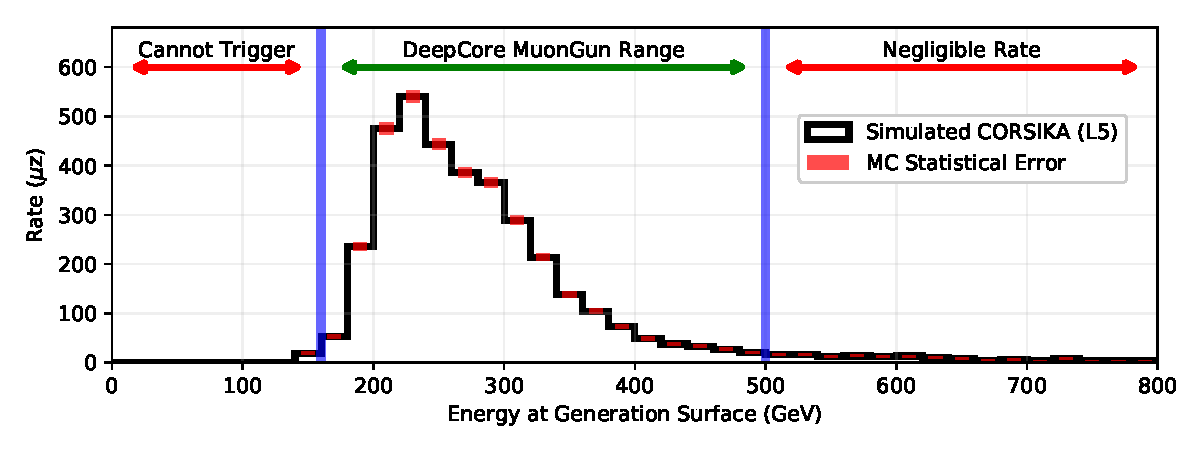
\includegraphics[width=0.8\textwidth]{corsika_mg_energy.pdf} 
\caption[The CORSIKA distribution at L5 used to select MuonGun's simulation range]{The distribution of CORSIKA muon energies at the MuonGun generation surface using GRECO Level 5 muon events. Very few events trigger below 160 GeV and less than 5\% of events occur beyond 500 GeV. These two energies set the bounds for the MuonGun generation. MuonGun simulation has also been produced and tested above 500 GeV, but no simulated events survived to Final Level in GRECO.}
\label{fig:muongun_energies}
\end{figure}

CORSIKA events observed in the GRECO selection at Level~5 (Section~\ref{sec:level5}), the last cut level with significant CORSIKA statistics available, are used to select an energy range for MuonGun simulation.
These events are shown in Figure~\ref{fig:muongun_energies}
The lower energy limit, 160~GeV, is selected by using CORSIKA simulation to identify the minimum energy required for a muon at the generation cylinder to reach and trigger the DeepCore detector.
A high energy limit on the MuonGun generation was set at 500~GeV, leaving the 5\% of the CORSIKA events above 500~GeV unsimulated.
The energy range selected, shown in Figure~\ref{fig:muongun_energies}, includes more than 95\% of the distribution of CORSIKA events.

The angular spectrum of the MuonGun simulation is created by setting a \emph{target cylinder} toward which the generated muon must intersect.
For this work, the DeepCore fiducial volume is used as a target, encompassing a cylinder with radius 150 meters and length 500 meters centered on the geometric center of DeepCore at x=(46.3, -34.9, -300). 

\begin{table}[]
\centering
\begin{tabular}{@{}llllll@{}}
\toprule
\multirow{2}{*}{Generator} & \multicolumn{2}{c}{Sim. Req.} & \multicolumn{2}{c}{Number of Events} & \multirow{2}{*}{$\epsilon$} \\
                           & CPU                  & GPU                  & Generation               &Final Level         &                             \\ \midrule
CORSIKA                    & 188.9 Years          & 48.75 Years          & 8 $\times 10^{12}$         & 284                    & 1.20                        \\
MuonGun         & 10.27 Years          & 12.11 Years          & 3 $\times 10^9$          & 2486                   & 111.08                      \\ \bottomrule
\end{tabular}
\caption{The computational requirements needed for the production of MuonGun simulation for DeepCore. The MuonGun simulation is nearly two orders of magnitude more efficient at producing statistics at Final Level in the appearance analysis.}
\label{tab:muongun_stats}
\end{table} 

A sample of muons was created using these settings of MuonGun and the resource requirements are shown in Figure~\ref{tab:muongun_stats}.
The efficiency improvement from changing to MuonGun is substantial, increasing from 1.20 CORSIKA events/year to 111.08 MuonGun events/year, an increase of nearly two orders of magnitude.

This simulation scheme has limitations. 
Because the target volume is small, events which do not enter DeepCore are not included in these MuonGun sets.
These events form a substantial background at early selection levels and cannot be ignored.
For this reason, CORSIKA muons are required for the development of selections and will be used in the Chapter~\ref{chapter:greco} until Level 5 (Section~\ref{sec:level5}).

The generated MuonGun statistics are useful for analyses at or near Final Level, where muons outside of DeepCore are no longer a dominant source of background.
The newly produced MuonGun statistics are used to model the muon background after Level 6 (Section~\ref{sec:level6}).

\section{Simulation Efficiency with KDE Prescales}
\label{sec:kde_filtering}
After processing to the Final Level of the GRECO event selection (see Chapter~\ref{chapter:greco}), the background MuonGun simulation retains 2486 simulated events of the original sample of 3$\times 10^9$ generated events.
The sample is sufficient for the search for tau neutrino appearance, but further improvements are possible.

\begin{figure}
\centering
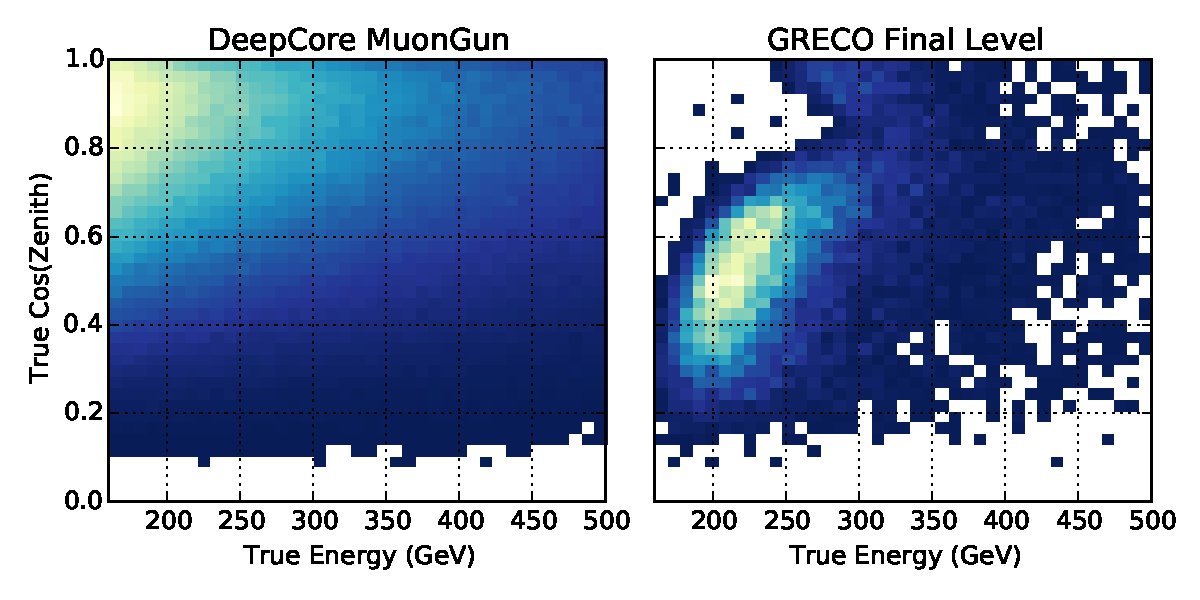
\includegraphics[width=0.9\textwidth]{energy_coszen_2.pdf}
\caption[Inefficiency in energy and zenith of the MuonGun generation spectrum]{The generated spectrum from MuonGun in energy and zenith angle compared to the muons reaching the Final Level of the GRECO event selection. Both distributions have been normalized to 1. The majority of events produced by MuonGun are downgoing and low energy. These events do not reach Final Level of the selection.}
\label{fig:e_coszen_nokde}
\end{figure}

While the previous section focused on improvements based on the simulation volume using MuonGun, inefficiencies still exist in the energy and zenith angle spectrum of the generated events.
This inefficiency is shown in Figure~\ref{fig:e_coszen_nokde}}.
The majority of the events produced by MuonGun are very downgoing (cos(zenith)$\approx$1) and low energy.
These events are noticeably absent from the Final Level sample. 

\begin{figure}
\centering
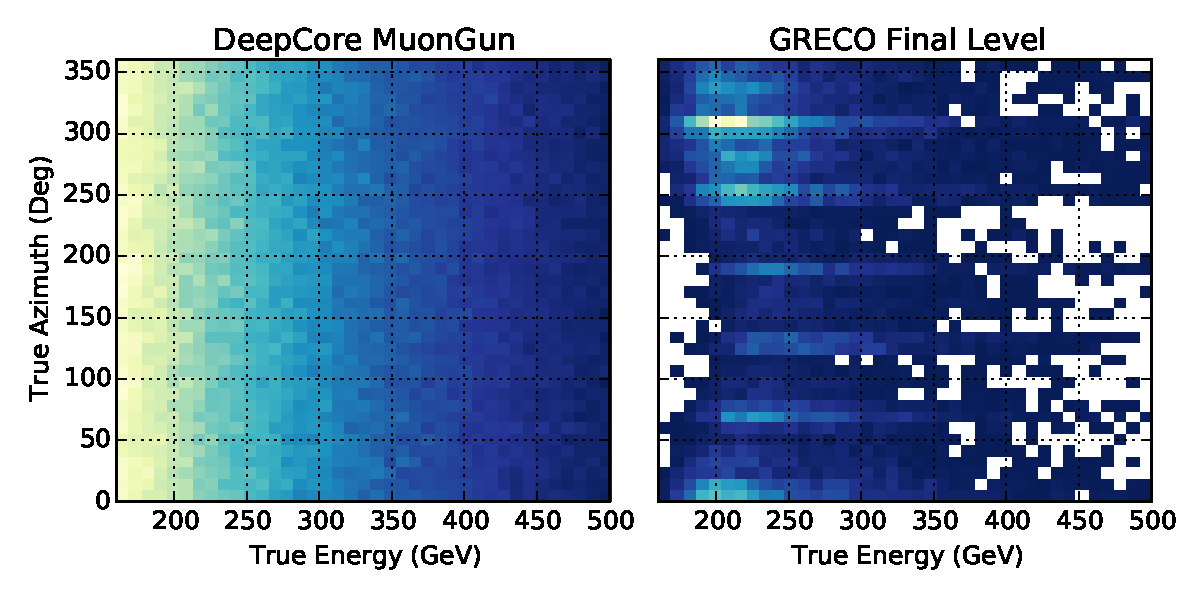
\includegraphics[width=0.9\textwidth]{energy_azimuth_2.pdf} 
\caption[Inefficiency in zenith and azimuth of the MuonGun generation spectrum]{The generated spectrum from MuonGun in energy and azimuthal angle compared to the muons reaching the Final Level of the GRECO event selection. Both distributions have been normalized to 1. Events in the Final Level sample are strongly biased in azimuth due to the geometry of the detector and the MuonGun production settings.}
\label{fig:e_coszen_nokde}
\end{figure}

In addition to the energy- and zenith-dependent effects, the GRECO selection exhibits strong azimuthal selection biases.
This arises due to three effects. 
The first is the offset between the center of IceCube (and therefore the center of the generation volume) at $(x,y)=(0,0)$ and DeepCore at $(x,y)=(46.3, -34.9)$.
Due to this offset, the distance required to reach the DeepCore fiducial volume at an azimuthal angle around 150 degrees is longer than the corresponding distance at 0 degrees.
This gives rise to an azimuthal effect appearing as a sinusoidal variation of the minimum generated energy of events at Final Level.

Another cause of azimuthal selection bias is the regular hexagonal structure of the IceCube volume, with long "corridors" through which muons may reach DeepCore without crossing any strings.
Cuts designed to look for hits in the veto region produce these azimuthal biases when muons traveling close to strings are more likely to be identified and removed than those further from strings (see Section~\ref{sec:level6}).

Finally, the DeepCore detector is not fully surrounded by an evenly distributed layer of strings.
This may be seen in Figure~\ref{fig:deepcore_layout}, where a layer of four strings is available for muon identification in the top left, but a layer of only three strings is available on the bottom right.
Events entering the detector from this direction are more likely to reach DeepCore without being tagged, resulting in a larger acceptance of events around 300 degrees.

In order to improve simulation statistics at Final Level, the existing MuonGun simulation scheme was modified to include an energy-, zenith-, and azimuthally-dependent prescale factor.
This approach, here referred to as a \emph{KDE prescale}, allows simulation to be produced with a known bias matching that of a given set of input files.

In this scheme, the \emph{kernal density estimator} (\emph{KDE}) from SciPy \cite{scipy} is applied to all remaining events at Final Level of the GRECO event selection. 
The KDE uses a Gaussian kernal to represent each event in energy, zenith, and azimuth. 
The resulting KDE is used to estimate the selection probability of muons in the Final Level of the GRECO sample.

\begin{figure}
\centering
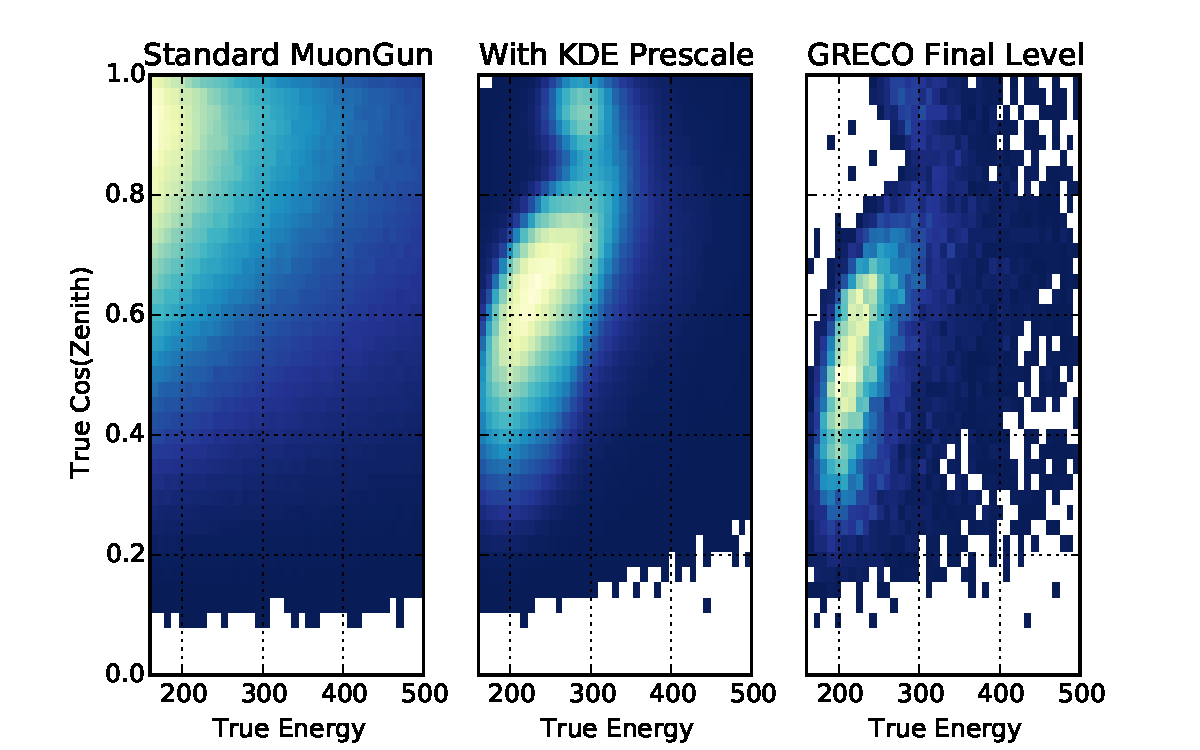
\includegraphics[width=0.9\textwidth]{energy_coszen.pdf} 
\caption[The MuonGun generation energy and zenith spectrum using the KDE Prescale]{The generated spectrum from the KDE prescaled MuonGun in energy and zenith angle compared to the muons reaching the Final Level of the GRECO event selection. Both distributions have been normalized to 1. The KDE prescale generation produces events which more closely model the event distributions from Final Level in the GRECO event selection.}
\label{fig:e_coszen_kde}
\end{figure}

\begin{figure}
\centering
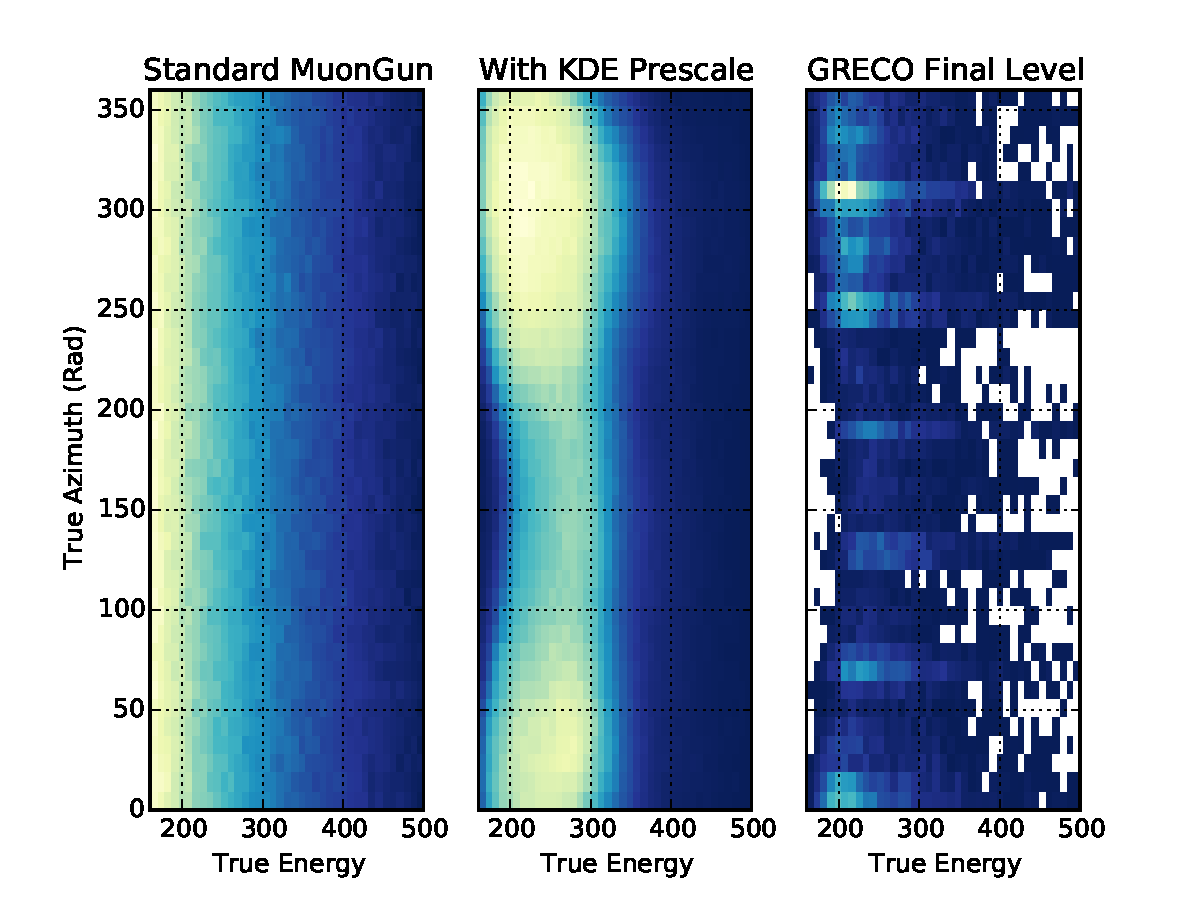
\includegraphics[width=0.9\textwidth]{energy_azimuth.pdf} 
\caption[The MuonGun generation energy and azimuthal spectrum using the KDE Prescale]{The generated spectrum from the KDE prescaled MuonGun in energy and azimuthal angle compared to the muons reaching the Final Level of the GRECO event selection. Both distributions have been normalized to 1. The KDE prescale generation produces events which more closely model the event distributions from Final Level in the GRECO event selection.}
\label{fig:e_azi_kde}
\end{figure}

In the new simulation scheme, shown in Figures~\ref{fig:e_coszen_kde} and \ref{fig:e_azi_kde}, an event is produced using standard settings for MuonGun generation described in the previous section.
Immediately following generation, the probability of the new event reaching Final Level is calculated from the KDE, with typical values 
of approximately $10^{-4}$ for a likely event and $10^{-9}$ or lower for unlikely events.
A prescale multiplicative factor of $10^5$ is used to set the overall probability scale.
The product, $p$, of the prescale factor and KDE probability is used in order to accept or reject events.
The value is interpreted as an acceptance probability and may not exceed 100\%.
Any values for which this may be the case are directly set to 100\%.

Using a random number generator, this $p$ factor is used to retain or reject the muon event.
The simulation then proceeds as normal, with photon propagation, detector simulation, triggering, and filtering.

\begin{table}[]
\centering
\begin{tabular}{@{}llllll@{}}
\toprule
\multirow{2}{*}{Generator} & \multicolumn{2}{c}{Sim. Req.} & \multicolumn{2}{c}{Number of Events} & \multirow{2}{*}{$\epsilon$} \\
                           & CPU                  & GPU                  & Generation               & Final Level         &                             \\ \midrule
CORSIKA                    & 188.9 Years          & 48.75 Years          & 8 $\times 10^{12}$         & 284                    & 1.20                        \\
MuonGun         & 10.27 Years          & 12.11 Years          & 3 $\times 10^9$          & 2486                   & 111.08                      \\
MuonGun+KDE            & 1.27 Years              & 214 Days             & 9 $\times 10^8$          & 3588                   & 1933.27                     \\ \bottomrule
\end{tabular}
\caption{The computational requirements and number of events for each muon generation scheme. The use of the KDE prescale improves the simulation efficiency by a factor of 50x compared to the DeepCore MuonGun simulation method described in Section~\ref{sec:muongun_deepcore}.}
\label{tab:kde_stats}
\end{table}

The results of experimental KDE prescale genereation are shown in Table~\ref{tab:kde_stats}.
By removing unlikely events early in the simulation chain, the required computational resources are further reduced compared to the general CORSIKA simulation sets produced by the IceCube collaboration.
While the number of events at Final Level is comparable to the MuonGun methods described in Section~\ref{sec:muongun_deepcore}, the required time for simulation is reduced to about 2 computation-years.

Further optimizations are possible at the expense of accuracy.
For example, the DOM oversizing methods described in Section~\ref{subsec:clsim} may be used to reduce the number of propagated photons.
Using $N_{OS}$=3, the GPU simulation requirements are further reduced by approximately 8x, leading to a total simulation efficiency of 2671.15.
The oversizing is known to cause a small bias in the simulated photon arrival time, potentially leading to bias in particle reconstructions.
Oversizing should be used with care in order to minimize or eliminate these biases.

The KDE prescale demonstrated here used only unweighted events due to limitations in the SciPy software.
The KDE therefore encodes some bias towards the production of low energy muons due to the soft spectral index of the MuonGun DeepCore generation.
Other implementations of multidimensional KDEs can accept event weights \cite{Thesis-Martin, Thesis-Schoenen}.
The use of these algorithms would be beneficial and remove some dependence on the generation characteristics of the source events used for building the KDE.

The simulation using KDE prescales is limited by the events used to form the KDE.
If too few events are used, the KDE may not adequately represent the shape of the underlying spectrum, leading to little gain in efficiency.
Likewise, if a region is underrepresented in the sample, the KDE may not describe the distribution of events in this region.
Care should be taken in order to check for unsimulated regions before using the KDE prescale to avoid these situations.

The use of the KDE prescale method shows substantial promise in improving simulation efficiency.
Work is ongoing within the IceCube collaboration at the time of this writing to investigate use of the method for DeepCore analyses.
If adopted, the improved simulation efficiency may allow future analyzers to significantly reduce the statistical uncertainty in the simulated background samples.
